\section{Antenna Characteristics}
\label{sec:calibration}

In this section, the array's antenna gains are measured and then analized.
The measured antenna gains can then directly be employed as weights for the backprojection algorithm,
resulting in a calibrated array.

\subsection{Setup}
To measure the antenna gains locationally, the sensor is mounted on a vertical rotating axis.
Rotating the axis allows a corner reflector to be observed from multiple angles, while retaining a fixed distance.
Doing this measures the antenna gain in azimuth;
to measure the antenna gain in elevation, the sensor is mounted on the same axis to rotate around its horizontal axis.
These two measurements are repeated for multiple reflector distances.

While the relative position of the rotating axis can be recorded with a decent resolution of around \SI{0.01}{\degree},
the absolute positioning of the reflector is hard to achieve with the same accuracy.
The sensor itself can however be used to improve positioning:
during setup, the phase of the peak caused by the reflector is displayed.
Mimimizing the phase differences between the array's channels ensures that the reflector be located at boresight.
These measurements are repeated with multiple distances of the relector.\\

The measurements are conducted outdoors to make room for longer distance measurements.
This however means that the recorded scene is not free of interference.

Several trees and brushes are located at the edge of the scene.
Extra interference and reflections are caused by the floor.
It is also not perfectly level, varying in height by up to \SI{1}{\meter},
which means that the reflector is not always exactly at the same height.
The sensor mount also causes some problems:
when the sensor is mounted on its inside,
the rotational axis passes exactly through the antenna plane,
but some shading is occurs when the reflector is on the same side as the sensor mount's diagonal reinforcement.
When the sensor is mounted on the outside,
the rotational axis is no longer in the antenna plane,
adding complexity and inaccuracy to the subsequent analysis.

\subsection{Results}
\subsubsection*{Preprocessing and Analysis}

The expected behavior is formulated in the signal model (see equation \ref{eqn:y_IF}ff.):
\begin{align}
    y_k(t=mT_s)                & =                  G_k(\vec r) e^{-j\dot\omega\tau_k mT_s},                 \\
    \text{where}\; G_k(\vec r) & = \frac{A_kA_S(\theta_S,\phi_S)}{R_{k}^2}  e^{-j\omega_0\tau_k + \varphi_k} \\
    \text{and}\;A_k :          & = A_{Tx,i} \cdot A_{Rx,j} \;\text{for}\;k=N_{Tx}i+j
\end{align}
A constant channel gain $A_k$, resulting from the transmitting and receiving antenna gains,
is attenuated with increasing distance, with $|G_k| \propto \frac{1}{R_{k}^2}$.
The effect of the angle of arrival on the gain is represented by the factor $A_S(\theta_S,\phi_S)$,
which is normalized such that $A_S(\theta_S,\phi_S) \in [0,1]$.
A constant channel phase offset $\varphi_k$ is set back proportionally to the time of flight $\tau_k = 2R_k/c$. \\

The goal of the subsequent analysis is twofold:
to extract all parameters of the above signal model while identifying and removing interference through processing.

Limiting the analysis to a single range bin will work towards both reducing interference and extracting parameters:
ideally, the DFT spectrum of the IF signal consists of just a single peak,
weighted with the locational gain $G_k(\vec r)$ (see eqn. \ref{eqn:y_fft}).
Thus, the parameters of the locational gain can be extracted if the correct bin $\hat \Omega$ is picked:
\begin{align}
    \hat \Omega                                               & = \dot \omega \tau_k(\vec r_S)T_s    \\
                                                              & = \dot \omega \frac{2R_k}{c}T_s      \\
    \Rightarrow \mathcal{F}_m\{y_k[m]\}(\Omega = \hat \Omega) & =    G_k(\vec r_S) \label{eqn:G_fft}
\end{align}

The relation between a range bin $\Omega$ and its corresponding range $r$ is
\begin{align}
    \Omega = r \cdot \frac{4N_{fft}\dot\omega}{c_0f_s}
\end{align}

\subsubsection*{Range Estimation}

In order to improve the accuracy of the subsequent analysis, the exact position of the reflector is estimated from the radar data.
To do this, numerical optimization is employed to find the parameter set $\hat R_s, \hat \theta_s, \hat \epsilon$ that minimizes the difference between
a range estimate $\hat R_{k,l}$ and the range spectral peak $R_{k,l}$ for all channels $k$ and recorded orientations $l$:
\begin{align}
    R_{k,l} = \text{arg } \underset{r}{\text{max}}\mathcal{F}_m\{y_{k,l}[m]\}\left(\Omega = \frac{N_{fft}r}{R_{max}}\right)
\end{align}

The range estimate $\hat R_{k,l}$ is determined geometrically from the distances of each channel's
transmit and receive antenna to the reflector. If the sensor is mounted to rotate in azimuth,
the range depends on the rotation angle $\theta_l $:

\begin{align}
    \hat R_{k,l}   & = \frac{\| \vec r_{TX,k} - \vec r_S(l) \|+\| \vec r_{RX,k} - \vec r_S(l) \|}{2}
    \\
    \vec{r}_{TX,k} & = \begin{bmatrix}
                           x_{TX,k} \\ y_{TX,k} \\ \hat \epsilon
                       \end{bmatrix},
    \vec r_{RX,k}       = \begin{bmatrix}
                              x_{RX,k} \\ y_{RX,k} \\ \hat \epsilon
                          \end{bmatrix},                                                                                        \\
    \vec r_S(l)    & = \begin{bmatrix}
                           (\hat R_S-\hat \epsilon) \text{sin}(\hat \theta_S-\theta_l) \\ 0 \\ (\hat R_S-\hat \epsilon) \text{cos}(\hat \theta_S-\theta_l)
                       \end{bmatrix},
\end{align}
If it is mounted to rotate in its elevation, the reflector appears to move depending on the rotation in elevation $\phi$.
For a given rotation angle $\phi_l$, it is located at
\begin{align}
    \vec r_S(l) & = \begin{bmatrix}
                        0 \\ (\hat R_S-\hat \epsilon) \text{sin}(\hat \phi_S-\phi_l) \\ (\hat R_S-\hat \epsilon) \text{cos}(\hat \phi_S-\phi_l)
                    \end{bmatrix},
\end{align}

In our setup, a signal is recorded with $\theta$ (or $\phi$, respectively) from \SIrange{0}{180}{\degree},
with the reflector located at roughly $R_S = \{2,8,18,32\}\si{\meter}$ and either $\theta_S = \SI{90}{\degree}$ or $\phi_S = \SI{90}{\degree}$.


With this, the loss $\mathcal L$ can be defined as the mean square difference between $\hat R$ and $R_{p}$,
the mean being computed as the average over all $K$ channels and $L$ sensor rotations:
\begin{align}
    \mathcal L(\hat R_s, \hat \theta_s, \hat \epsilon)
    = \frac{1}{KL}\sum_{l=0}^{L-1} \sum_{k=0}^{K-1} ( R_{k,l} - \hat  R_{k,l}(\hat R_s, \hat \theta_s, \hat \epsilon))^2
\end{align} \\

Figure \ref{fig:reflpos_estimate} shows the result of 100 iterations at an adaption rate of 0.05 at the example of three different channels,
comparing the measured spectral peaks (shown as points) to the estimated position (dotted line) of the reflector.
Only a subset of orientations is used for the estimate,
namely \SI{-50}{\degree} $<\theta_l-$\SI{90}{\degree}$<$ \SI{20}{\degree}. \\


For the first three measurements, the peak location oscillates around the estimate by \SIrange[range-units=single]{1}{2}{\cm}.
The root mean square error is reduced to \SI{11}{\mm}
The fourth measurement has higher noise, with no clear line being visible in the spectral peaks.

\begin{figure}
    \centering
    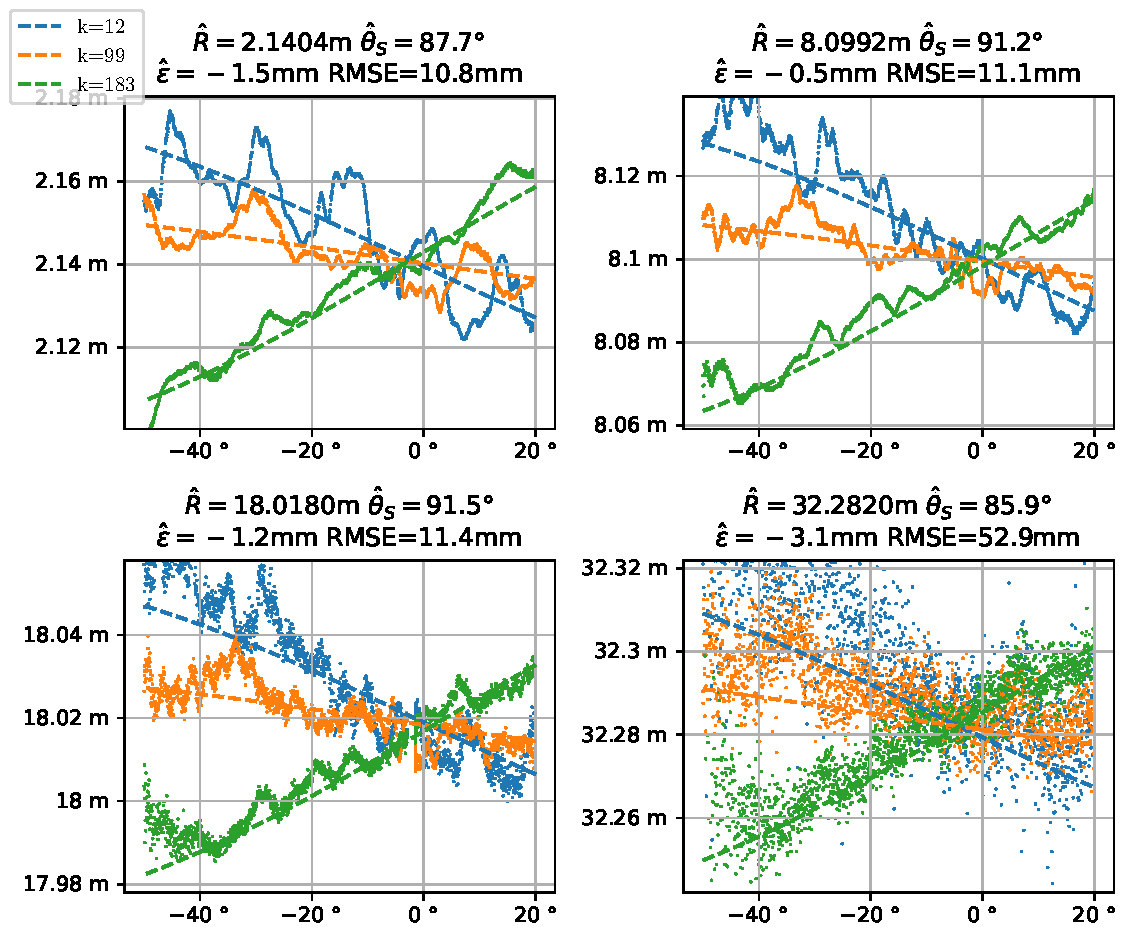
\includegraphics[width=\textwidth]{../figures/reflpos_estimate.pdf}
    \caption{Example Optimization Results}
    \label{fig:reflpos_estimate}
\end{figure}

\subsubsection*{Amplitude}
First, the recorded amplitudes are analyzed, beginning with the influence of the angle of arrival.
To do this, each channel's range FFT spectrum's amplitude is evaluated at the respective calculated peak location $\hat \Omega$,
and then normalized by dividing it by its maximum.

The first parameters to extract are the three factors $A_{Tx}$, $A_{Rx}$ and $A_S(\theta_S,\phi_S)$.
Since the angle of arrival's impact has been constrained to $[0,1]$, we know that
\begin{align}
    \underset{\theta,\phi}{\text{max}} |G_k(R,\theta,\phi)|  = \frac{A_k}{R^2} \label{eqn:max_G}
\end{align} \\
With that, an estimate of the channel gain $A_k$ at exactly \SI{1}{\meter} can be obtained via linear regression.
An example linear regression is shown in figure \ref{fig:ch0_amp_linreg},
and the resulting estimates with their standard deviations are summarized in figure \ref{fig:amp_linreg}. \\

\begin{figure}
    \centering
    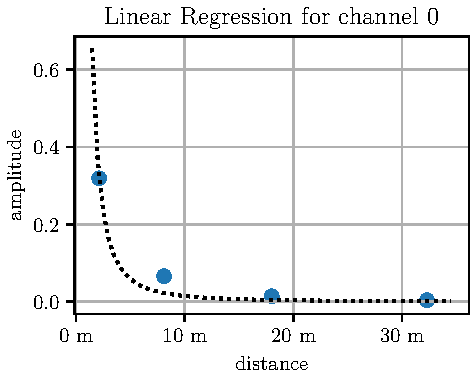
\includegraphics[width=0.6\textwidth]{../figures/ch0_amplitude_linreg.pdf}
    \caption{Example Channel Gain Linear Regression}
    \label{fig:ch0_amp_linreg}
\end{figure}
\begin{figure}
    \centering
    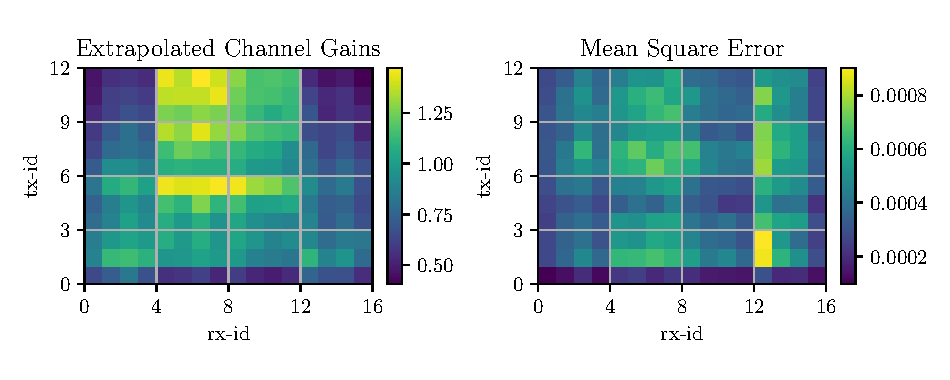
\includegraphics[width=\textwidth]{../figures/amplitude_linreg.pdf}
    \caption{Example Channel Gain Linear Regression}
    \label{fig:amp_linreg}
\end{figure}
To now separate the estimated channel gains $\hat A_k$ into individual antenna gains $\hat A_{Tx,i}$ and $\hat A_{Rx,j}$,
receive antenna 0 is chosen as a reference, i.e. $\hat A_{Rx,0} :=1$.
All measurements with receive antenna 0 are therefor used to directly measure the transmit antenna gains:
\begin{align}
    \hat A_{Tx,i}  = \hat A_{k=N_{Tx}i} \text{ for }i=0 \dots N_{Tx-1}
\end{align}
With that, the least-squares estimate of the receive antenna gains becomes
\begin{align}
    \hat A_{Rx,j} = \frac{1}{N_{Tx}} \sum_{i=0}^{N_{Tx}-1} \frac{\hat A_{k=N_{Rx}i+j}}{\hat A_{k=N_{Rx}i}}
\end{align} \\

\begin{figure}
    \centering
    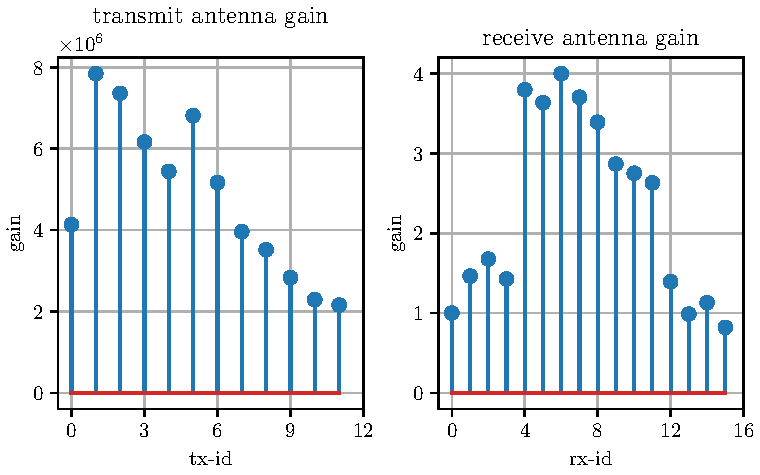
\includegraphics[width=0.8\textwidth]{../figures/antenna_gains.pdf}
    \caption{Estimated Antenna Gains}
    \label{fig:antenna_gains}
\end{figure}
The resulting antenna gains are shown in figure \ref{fig:antenna_gains}.
Further measurements would be required to reduce the substantial error bars.
A next step would consist of a measurement setup with a linear axis moving the reflector,
which would generate substantially more sample points for the linear regression. \\

Having estimated channel gains and outlined a method for separating them into the transmit and receive antenna gains,
we can now turn to analysing the angle-of-arrival characteristics.
Assuming the omptimal range bin $\hat \Omega$ is evaluated each time, we get
\begin{align}
    \left|\mathcal{F}_m\{y_k[m]\}(\Omega = \hat \Omega)  \right| =  \frac{A_kA_S(\theta_S,\phi_S)}{R_{k}^2} =  |G_k(\vec r_S)|
\end{align}
Dividing that by the maximum gain (\ref{eqn:max_G}) yields
\begin{align}
    \frac {|G_k(\vec r_S)|}{\underset{\theta,\phi}{\text{max}} |G_k(R,\theta,\phi)|}  = A_S(\theta,\phi)
\end{align}

% Just like the channel gain $A_k$ can be separated into transmit and receive antenna gains, 
% the directivity $A_S(\theta,\phi)$ can be separated into transmit and receive antenna directivities, 
% again using receive antenna 0 as a reference.
\begin{figure}
    \centering
    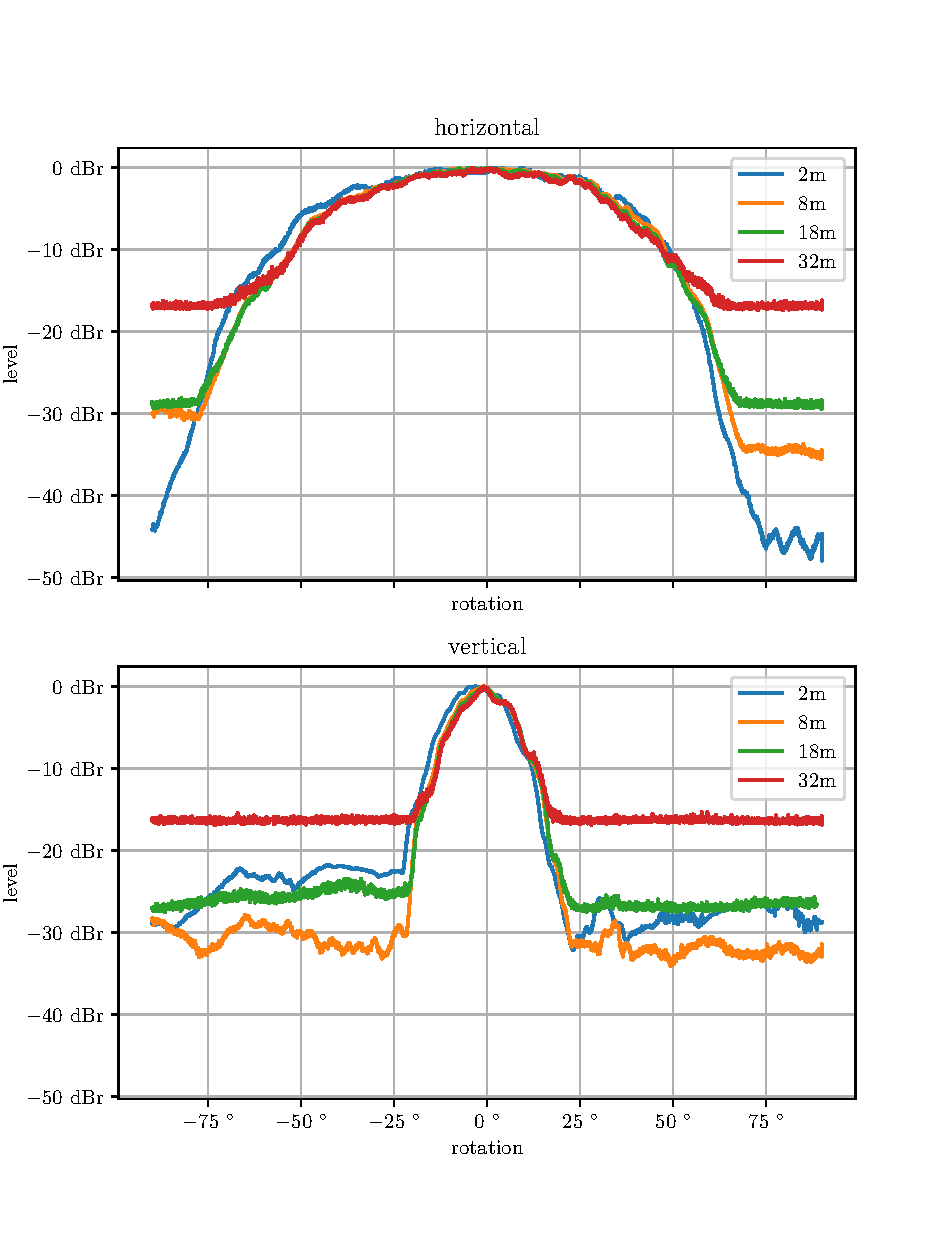
\includegraphics[width=\textwidth]{../figures/mean_amp.pdf}
    \caption{Mean Amplitude for multiple reflector distances}
    \label{fig:mean_amp}
\end{figure}

Figure \ref{fig:mean_amp} provides an overview by displaying the mean channel characteristic for each measurement.
It can be seen that the gain is strongest when the target is directly in boresight,
tapering off when the target is off-center. The reduction in gain is stronger when the target
moves off to the side in the elevation, than in azimuth. While the target remains stronger
than background noise up until an azimuth angle of around \SIrange{-75}{+75}{\degree},
it can only be seen in an elevation angle sector from \SIrange{-25}{+25}{\degree}.

The graphs of the horizontal measurements appear slightly asymmetrical, an effect which is investigated in the following. \\

\begin{figure}
    \centering
    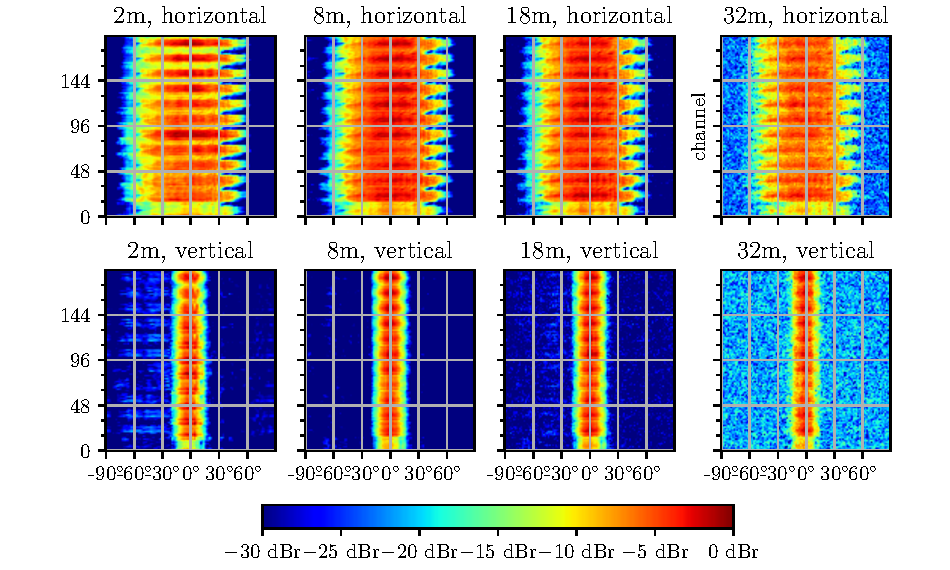
\includegraphics[width=\textwidth]{../figures/channel_amp.pdf}
    \caption{Channel-wise amplitude for multiple distances}
    \label{fig:chan_amp}
\end{figure}

A possible explanation for the asymmetry is the sensor mount,
which protrudes out on the right side of the array,
attenuating the signal received by antennas on that side when the reflector is behind said protrusion.

Investigating the individual channel gains (c.f. \ref{fig:chan_amp}) gives a first indication:
the asymmetry is most pronounced when comparing the range of \SIrange{30}{60}{\degree}
to its counterpart of \SIrange{-30}{-60}{\degree} for the horizontal measurements.
Namely, in the former range, the gain seems to oscillate every 16 channels.

\begin{figure}
    \centering
    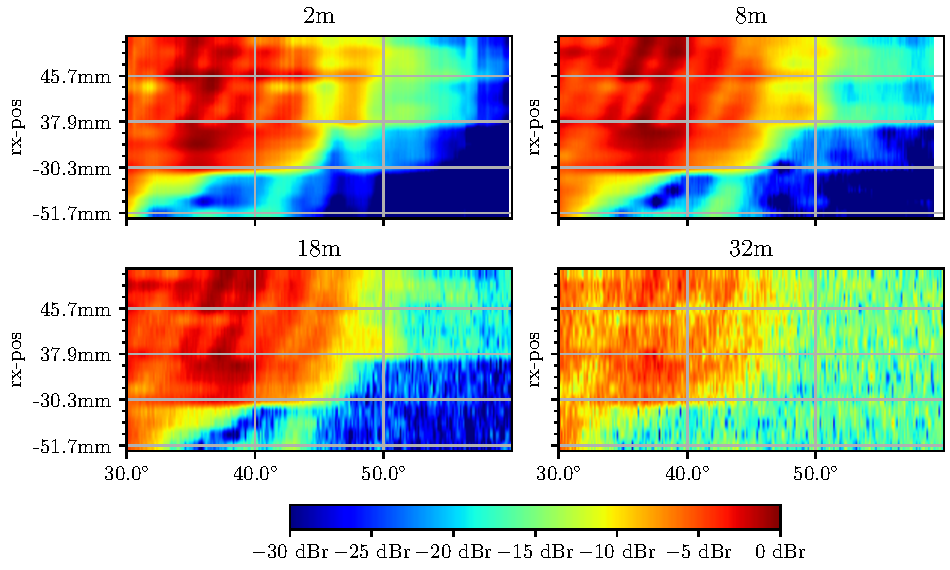
\includegraphics[width=\textwidth]{../figures/channel_amp_tx0.pdf}
    \caption{Channel-wise amplitude for multiple distances, channels arranged by Rx antenna position, only Tx antenna 0 active}
    \label{fig:chan_amp_tx0}
\end{figure}

To explore further, figure \ref{fig:chan_amp_tx0} zooms in on one period.
It shows the channel gain of the horizontal measurements for angles \SIrange{30}{60}{\degree}
of the channels in which transmit antenna 0 is active, arranged by the horizontal position of the receive antenna, from left to right.
It can now be seen that the channel gain of antennas closer to the sensor mount's protrusion drops
in amplitude at lower angles than that of the antennas further away from it,
confirming that the sensor mount is responsible for the asymmetry.
To get a more accurate estimate of the channel characteristics,
the measurements have to be repeated with the sensor mounted on the outside.\\

With this, the individual antenna gains and the channel characteristics have been extracted from the data.
In the next step, the recorded phases are analyzed.

\subsubsection*{Phase}
The first step in extracting the phase parameters from the recorded data is yet again
evaluating the signal's DFT phase at the optimum range bin $\hat \Omega$,
which according to (\ref{eqn:G_fft}) yields
\begin{align}
    \text{arg} \mathcal{F}_m\{y_k[m]\}(\Omega = \hat \Omega) & =    \text{arg}G_k(\vec r_S)                  \\
                                                             & = \omega_0\tau_k + \varphi_k                  \\
    \text{with } \varphi_k                                   & = \varphi_{Tx,i}+\varphi_{Rx,j},  k=N_{rx}i+j \\
    \text{ and } \tau_k                                      & = \frac{2r_S}{c_0}
\end{align}
Ideally, the channel phase offset should be constant for every


\subsubsection*{Excentricity Optimiziation}

\subsubsection*{Antenna Separation}

\subsubsection*{Conclusion}